\section{Empirical Results}

\subsection{Descriptive Statistics and Market Microstructure}

The VN-Index daily panel spans 2,498 trading days over ten years (2015--2024), yielding 2,497 one-step-ahead forecasting observations. Table \ref{tab:descriptive_stats} summarizes the return and sentiment distributions.

\begin{table}[htbp]
    \centering
    \caption{Descriptive Statistics of VN-Index Daily Returns and News Sentiment}
    \label{tab:descriptive_stats}
    \begin{tabular}{lccccc}
        \toprule
        Series & Mean & Std. Dev. & Minimum & Maximum & Kurtosis \\
        \midrule
        VN-Index Returns (\%) & 0.0338 & 1.1390 & -6.9076 & 4.8600 & 7.5934 \\
        Article Sentiment Score & 0.4526 & 0.3694 & -0.9622 & 0.9991 & -- \\
        Daily Article Count & 34.5 & 28.7 & 0 & 386 & -- \\
        \bottomrule
    \end{tabular}
\end{table}

\subsubsection{Return Dynamics and Volatility Clustering}

The VN-Index exhibits significant departure from normality. Daily returns have a kurtosis of 7.59, well above the Gaussian benchmark of 3.0, indicating heavy tails and extreme-event clustering. A Jarque-Bera test strongly rejects normality ($JB = 2554.1$, $p < 0.001$). This leptokurtosis reflects the retail-investor-dominated nature of the market: retail investors' herding behavior amplifies both rallies and crashes relative to what normal-distribution pricing models predict.

\begin{figure}[htbp]
    \centering
    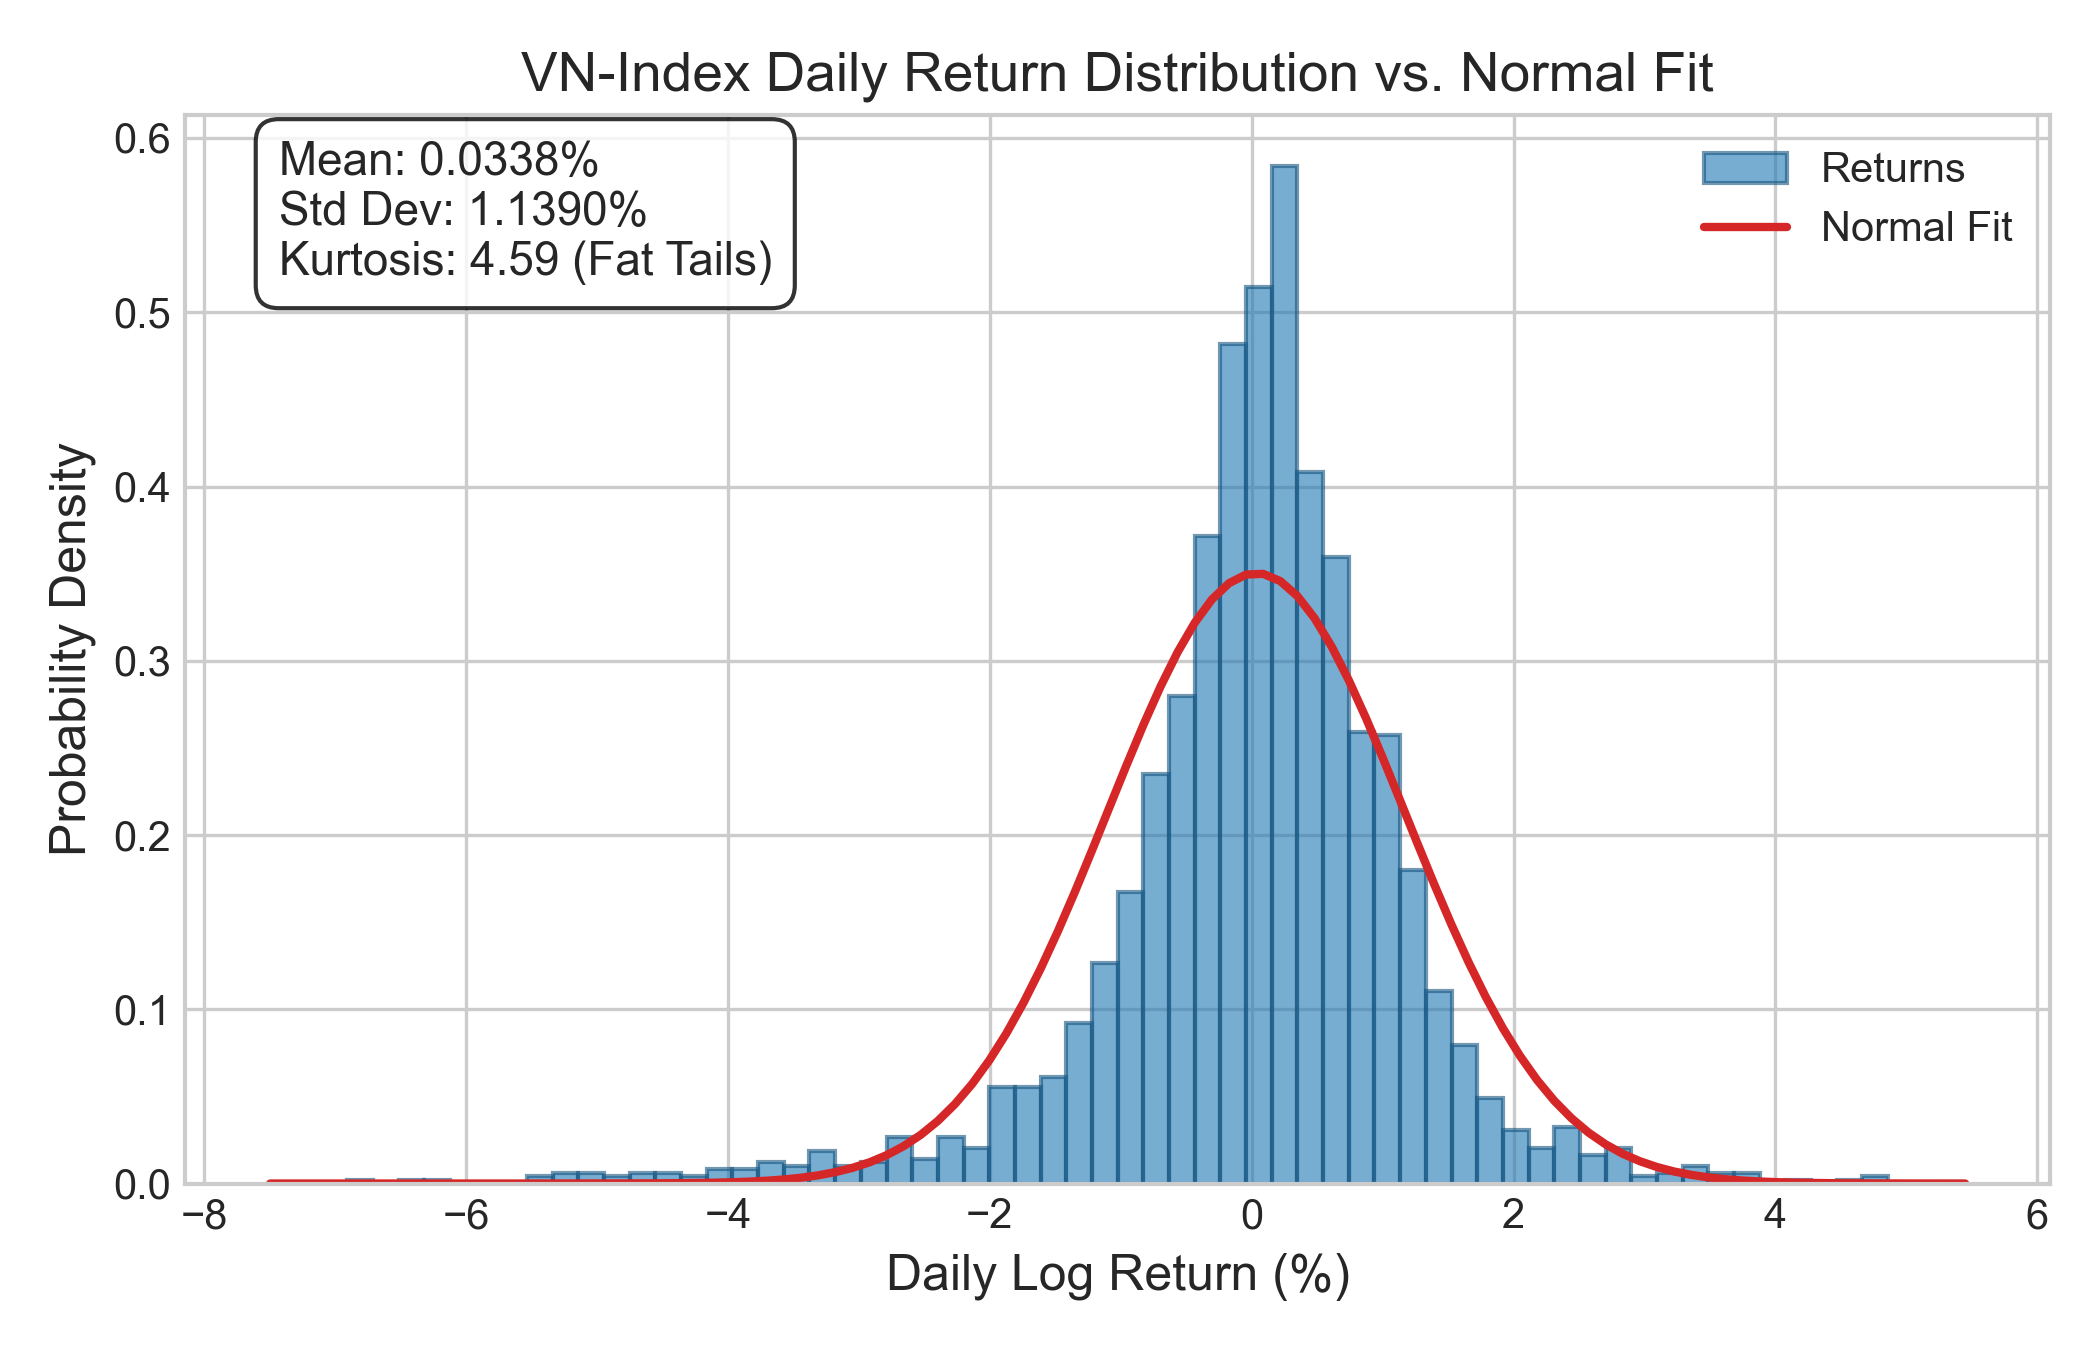
\includegraphics[width=0.75\textwidth]{figures/return_distribution.png}
    \caption{VN-Index Daily Return Distribution vs. Normal Fit}
    \label{fig:return_distribution}
\end{figure}

A Ljung-Box test reveals significant return autocorrelation ($Q(5) = 14.48$, $p = 0.0128$), suggesting mean-reverting or momentum effects on short horizons. More critically, squared returns exhibit extremely strong autocorrelation ($Q(5) = 414.46$, $p < 0.001$; $Q(10) = 681.83$, $p < 0.001$), confirming strong volatility clustering. Figure \ref{fig:vol_clustering} visualizes conditional variance over time, with major spikes during the COVID-19 crash (March 2020) and the 2022 domestic liquidity shock. These clustering patterns and regime shifts motivate GARCH modeling, which captures the temporal autocorrelation in squared residuals through the persistence parameter $\beta$.

\begin{figure}[htbp]
    \centering
    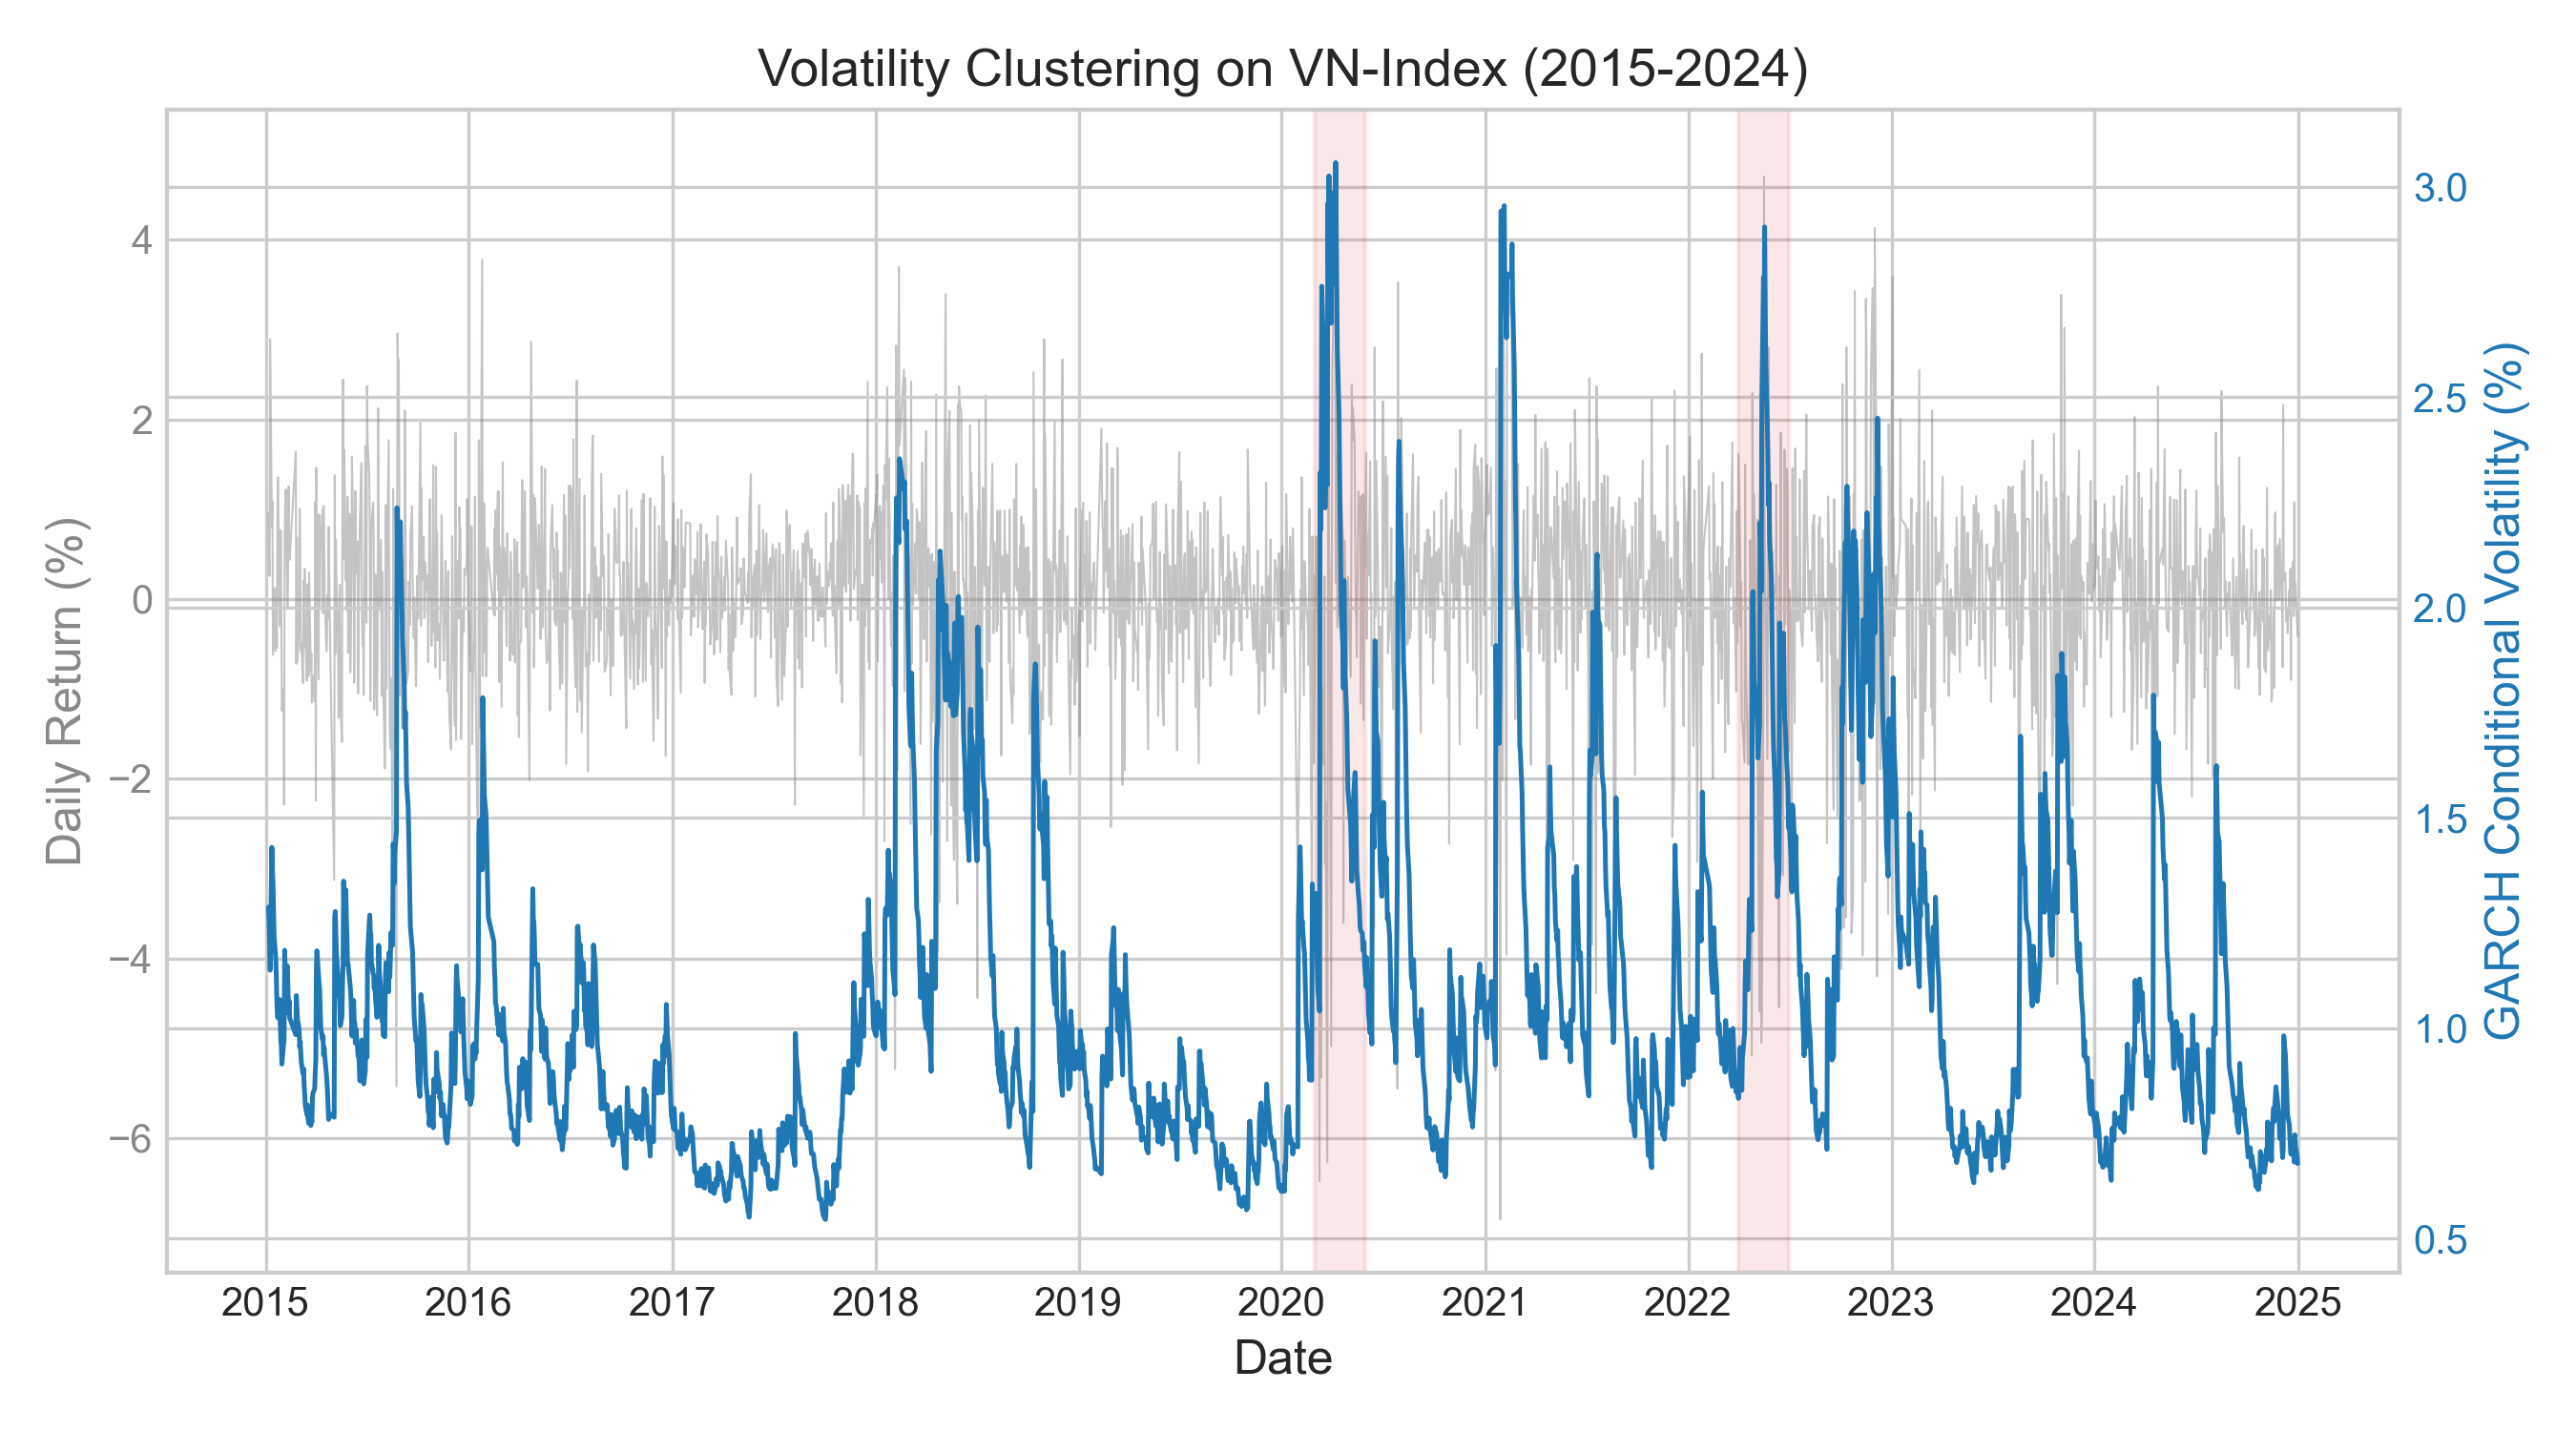
\includegraphics[width=0.9\textwidth]{figures/vol_clustering.png}
    \caption{VN-Index Conditional Volatility and Return Clustering (2015--2024)}
    \label{fig:vol_clustering}
\end{figure}

\subsubsection{News Sentiment Distribution and Media Bias}

The sentiment corpus of 86,179 articles reveals pronounced positive bias. The mean sentiment score is 0.4526 (on a scale of $-1$ to $+1$), indicating systematic upward skew in Vietnamese financial journalism. Under a standard classification threshold of $\pm 0.05$, positive articles comprise 84.34\% of the corpus (72,686 articles), while negative articles represent only 12.04\% (10,380 articles), with neutral articles making up 3.61\% (3,113 articles). Figure \ref{fig:sentiment_distribution} shows the highly skewed distribution.

\begin{figure}[htbp]
    \centering
    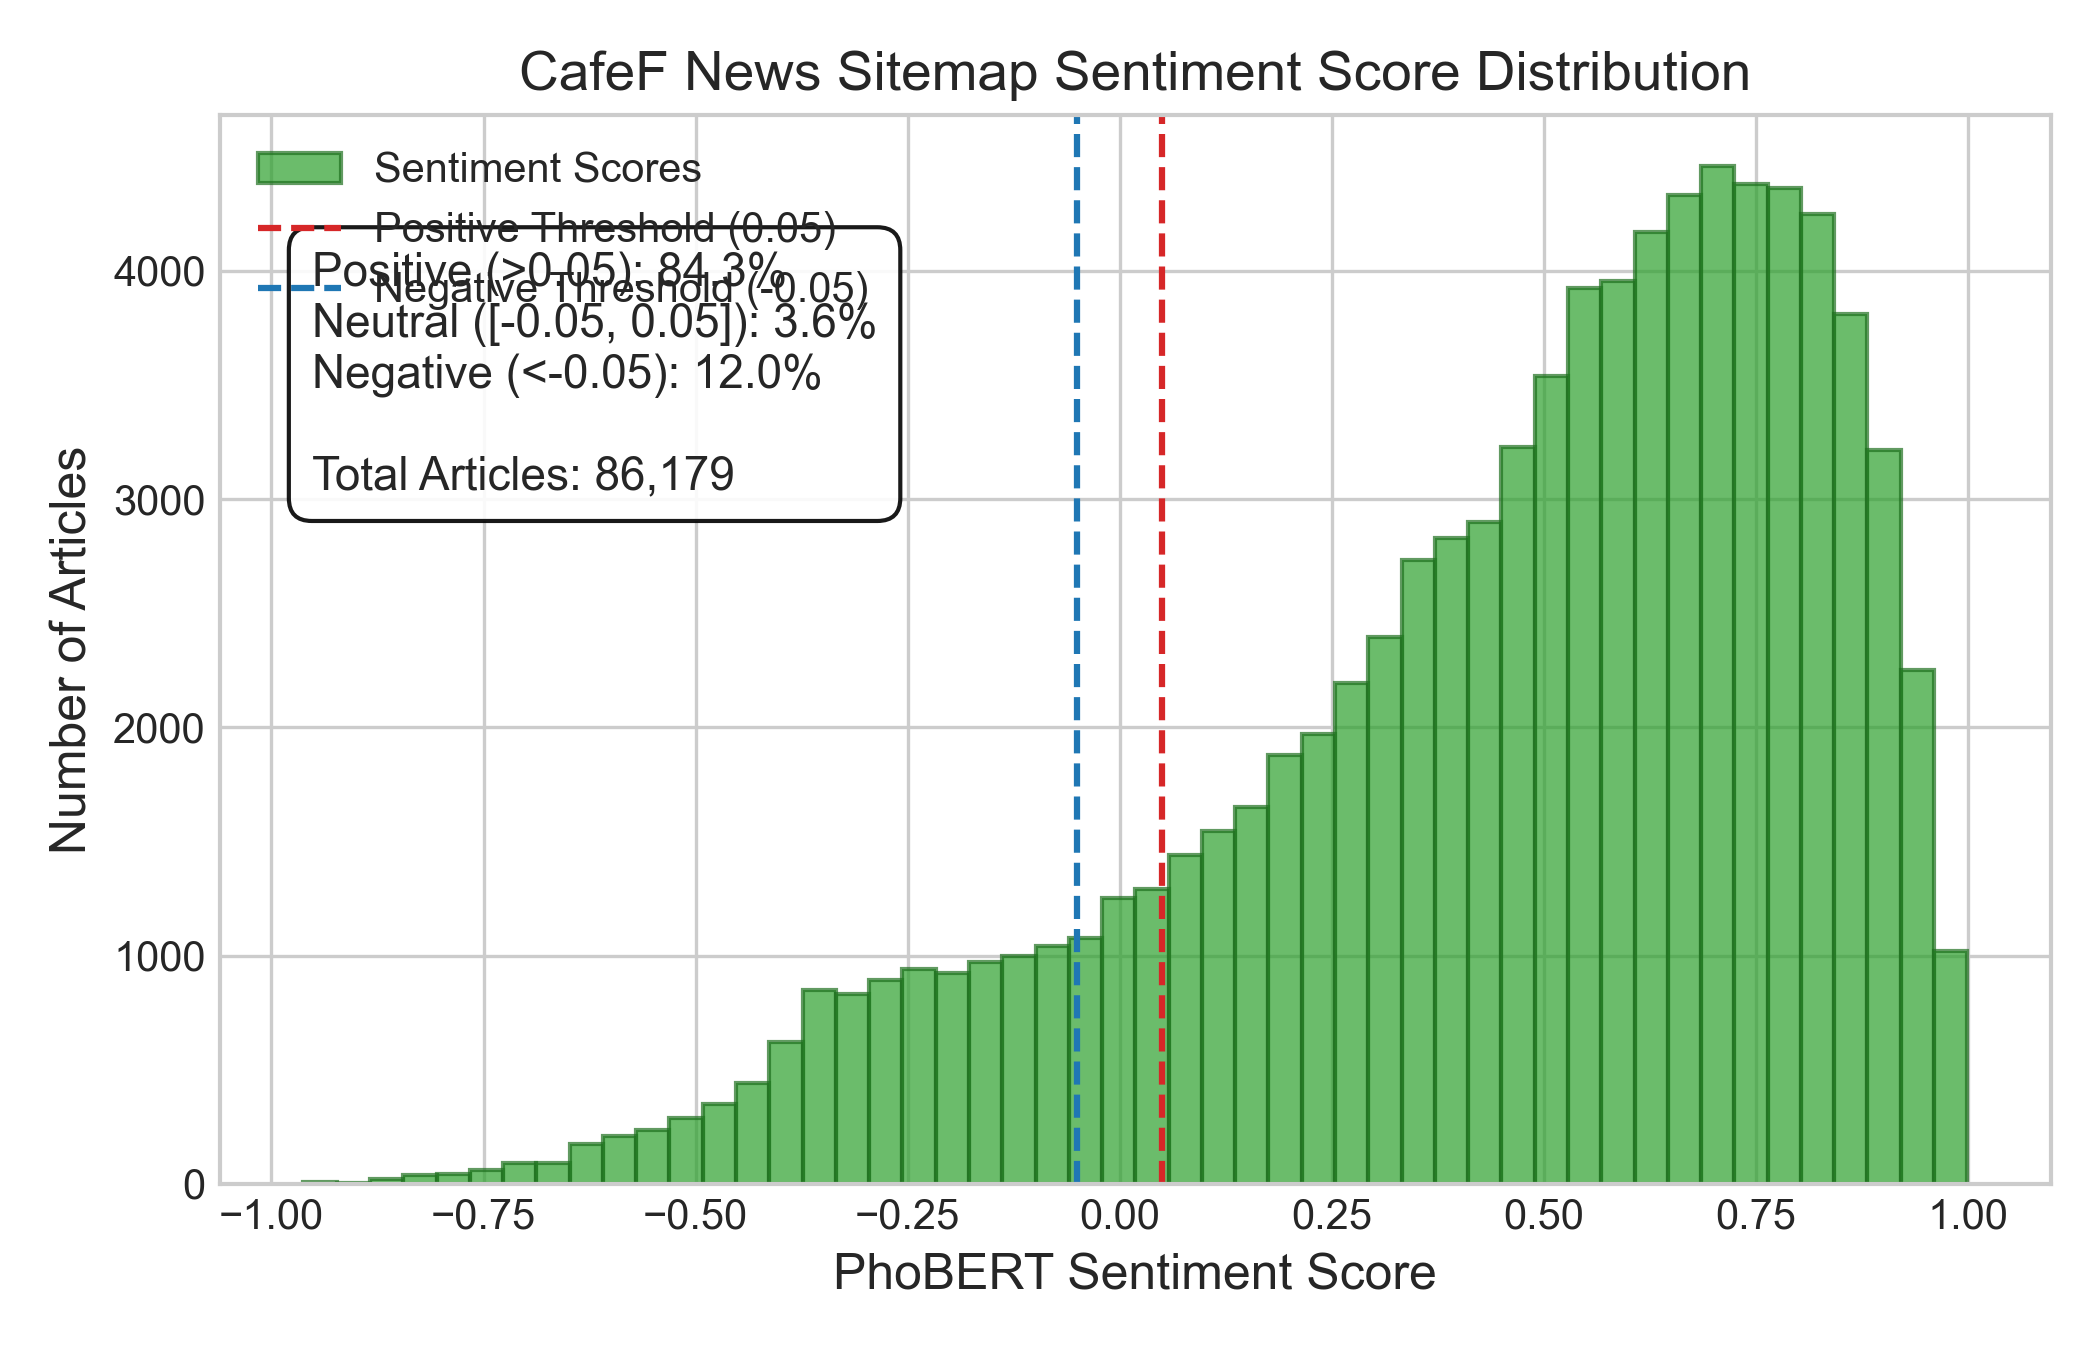
\includegraphics[width=0.75\textwidth]{figures/sentiment_distribution.png}
    \caption{Distribution of Article Sentiment Scores: Strong Positive Bias in Vietnamese Financial Media}
    \label{fig:sentiment_distribution}
\end{figure}

This positive bias has three implications. First, it reflects media economics: financial news outlets cater to retail investors who have a strong preference for positive narratives, creating demand for optimistic framing. Second, it raises the signal-to-noise ratio: negative news, being rare and extreme, may have disproportionate informational weight and market impact. Third, it explains why models using simple mean sentiment often perform poorly—the unconditional mean is high and non-informative; the variation (negative days vs. baseline positive days) carries information. This motivates studying \textit{negative sentiment share} separately.

Daily article volume averages 34.5 articles per day ($\sigma = 28.7$), with maximum of 386 articles on high-intensity news days. Only 4 of 2,498 trading days (0.16\%) have zero aligned articles, confirming that CafeF provides continuous, reliable daily news coverage.

\subsubsection{GARCH(1,1) Baseline Specification and Diagnostics}

We fit a Gaussian AR(1)-GARCH(1,1) model on the training data (2015--2021, 1,753 observations). Maximum likelihood estimation yields:
$$\omega = 0.0258, \quad \alpha = 0.1026, \quad \beta = 0.8810$$

The persistence parameter $\alpha + \beta = 0.9836$ is close to unity, indicating extremely high volatility persistence. This high persistence is economically meaningful: a volatility shock today has lasting effects on predicted variance for weeks or months. The high $\beta$ reflects the dominance of recent history (lagged variance) over recent shocks (lagged squared residuals) in predicting next-period variance, consistent with international equity market patterns.

\textit{Diagnostic tests:} The Ljung-Box test on squared standardized residuals yields p-values of 0.9796 (lag 5) and 0.4956 (lag 10), well above the 5\% significance level. We fail to reject the null of no remaining ARCH effects, confirming that the GARCH(1,1) specification successfully captures linear conditional heteroskedasticity. The model is thus well-specified for its intended purpose: serving as a parsimonious baseline for Stage 1 of the hybrid architecture.

\subsection{Out-of-Sample Forecast Performance}

Table \ref{tab:forecasting_results} compares the one-step-ahead forecast accuracy of the baseline GARCH(1,1) against the hybrid GARCH-LSTM model on the held-out test window (2022--2024, 744 observations).

\begin{table}[htbp]
    \centering
    \caption{Out-of-Sample Volatility Forecast Performance: GARCH Baseline vs. Hybrid GARCH-LSTM}
    \label{tab:forecasting_results}
    \begin{tabular}{lccccc}
        \toprule
        Model & RMSE & MAE & MAPE & DM $t$-stat & $p$-value \\
        \midrule
        GARCH(1,1) Baseline & 0.004701 & 0.003828 & 79.24\% & -- & -- \\
        GARCH-LSTM & 0.004020 & 0.002628 & 41.21\% & 3.420 & 0.000627 \\
        \textbf{Improvement (\%)} & \textbf{-14.48\%} & \textbf{-31.35\%} & \textbf{-48.00\%} & & \\
        \bottomrule
    \end{tabular}
\end{table}

The hybrid model achieves economically substantial forecast improvements across all error metrics. RMSE drops from 0.004701 to 0.004020, a 14.48\% improvement. MAE decreases by 31.35\% (from 0.003828 to 0.002628), indicating the hybrid model's conditional volatility forecasts are systematically closer to realized values. MAPE plummets from 79.24\% to 41.21\% (a 48.00\% improvement), the most dramatic gain. The MAPE improvement reflects the hybrid model's ability to adapt to rapidly changing volatility levels—it makes proportionally smaller errors whether volatility is high or low, whereas the baseline GARCH struggles with the wide range of volatility magnitudes observed in the test window.

\textit{Statistical significance:} A Diebold-Mariano test with Newey-West adjustment for autocorrelated forecast errors yields $t_{DM} = 3.420$ ($p = 0.000627$), rejecting equal predictive accuracy at the 99.9\% confidence level. This decisive rejection confirms that the improvements are not sampling variation but genuine out-of-sample forecasting power.

Figure \ref{fig:forecast_comparison} plots the time series of realized, GARCH-forecasted, and hybrid-forecasted volatility over the test window. Visual inspection reveals that the hybrid model's forecasts track realized volatility more closely, particularly capturing rapid volatility spikes and declines that the baseline GARCH smooths over. This adaptiveness is consistent with the hypothesis that sentiment variables encode real-time information about market sentiment shifts.

\begin{figure}[htbp]
    \centering
    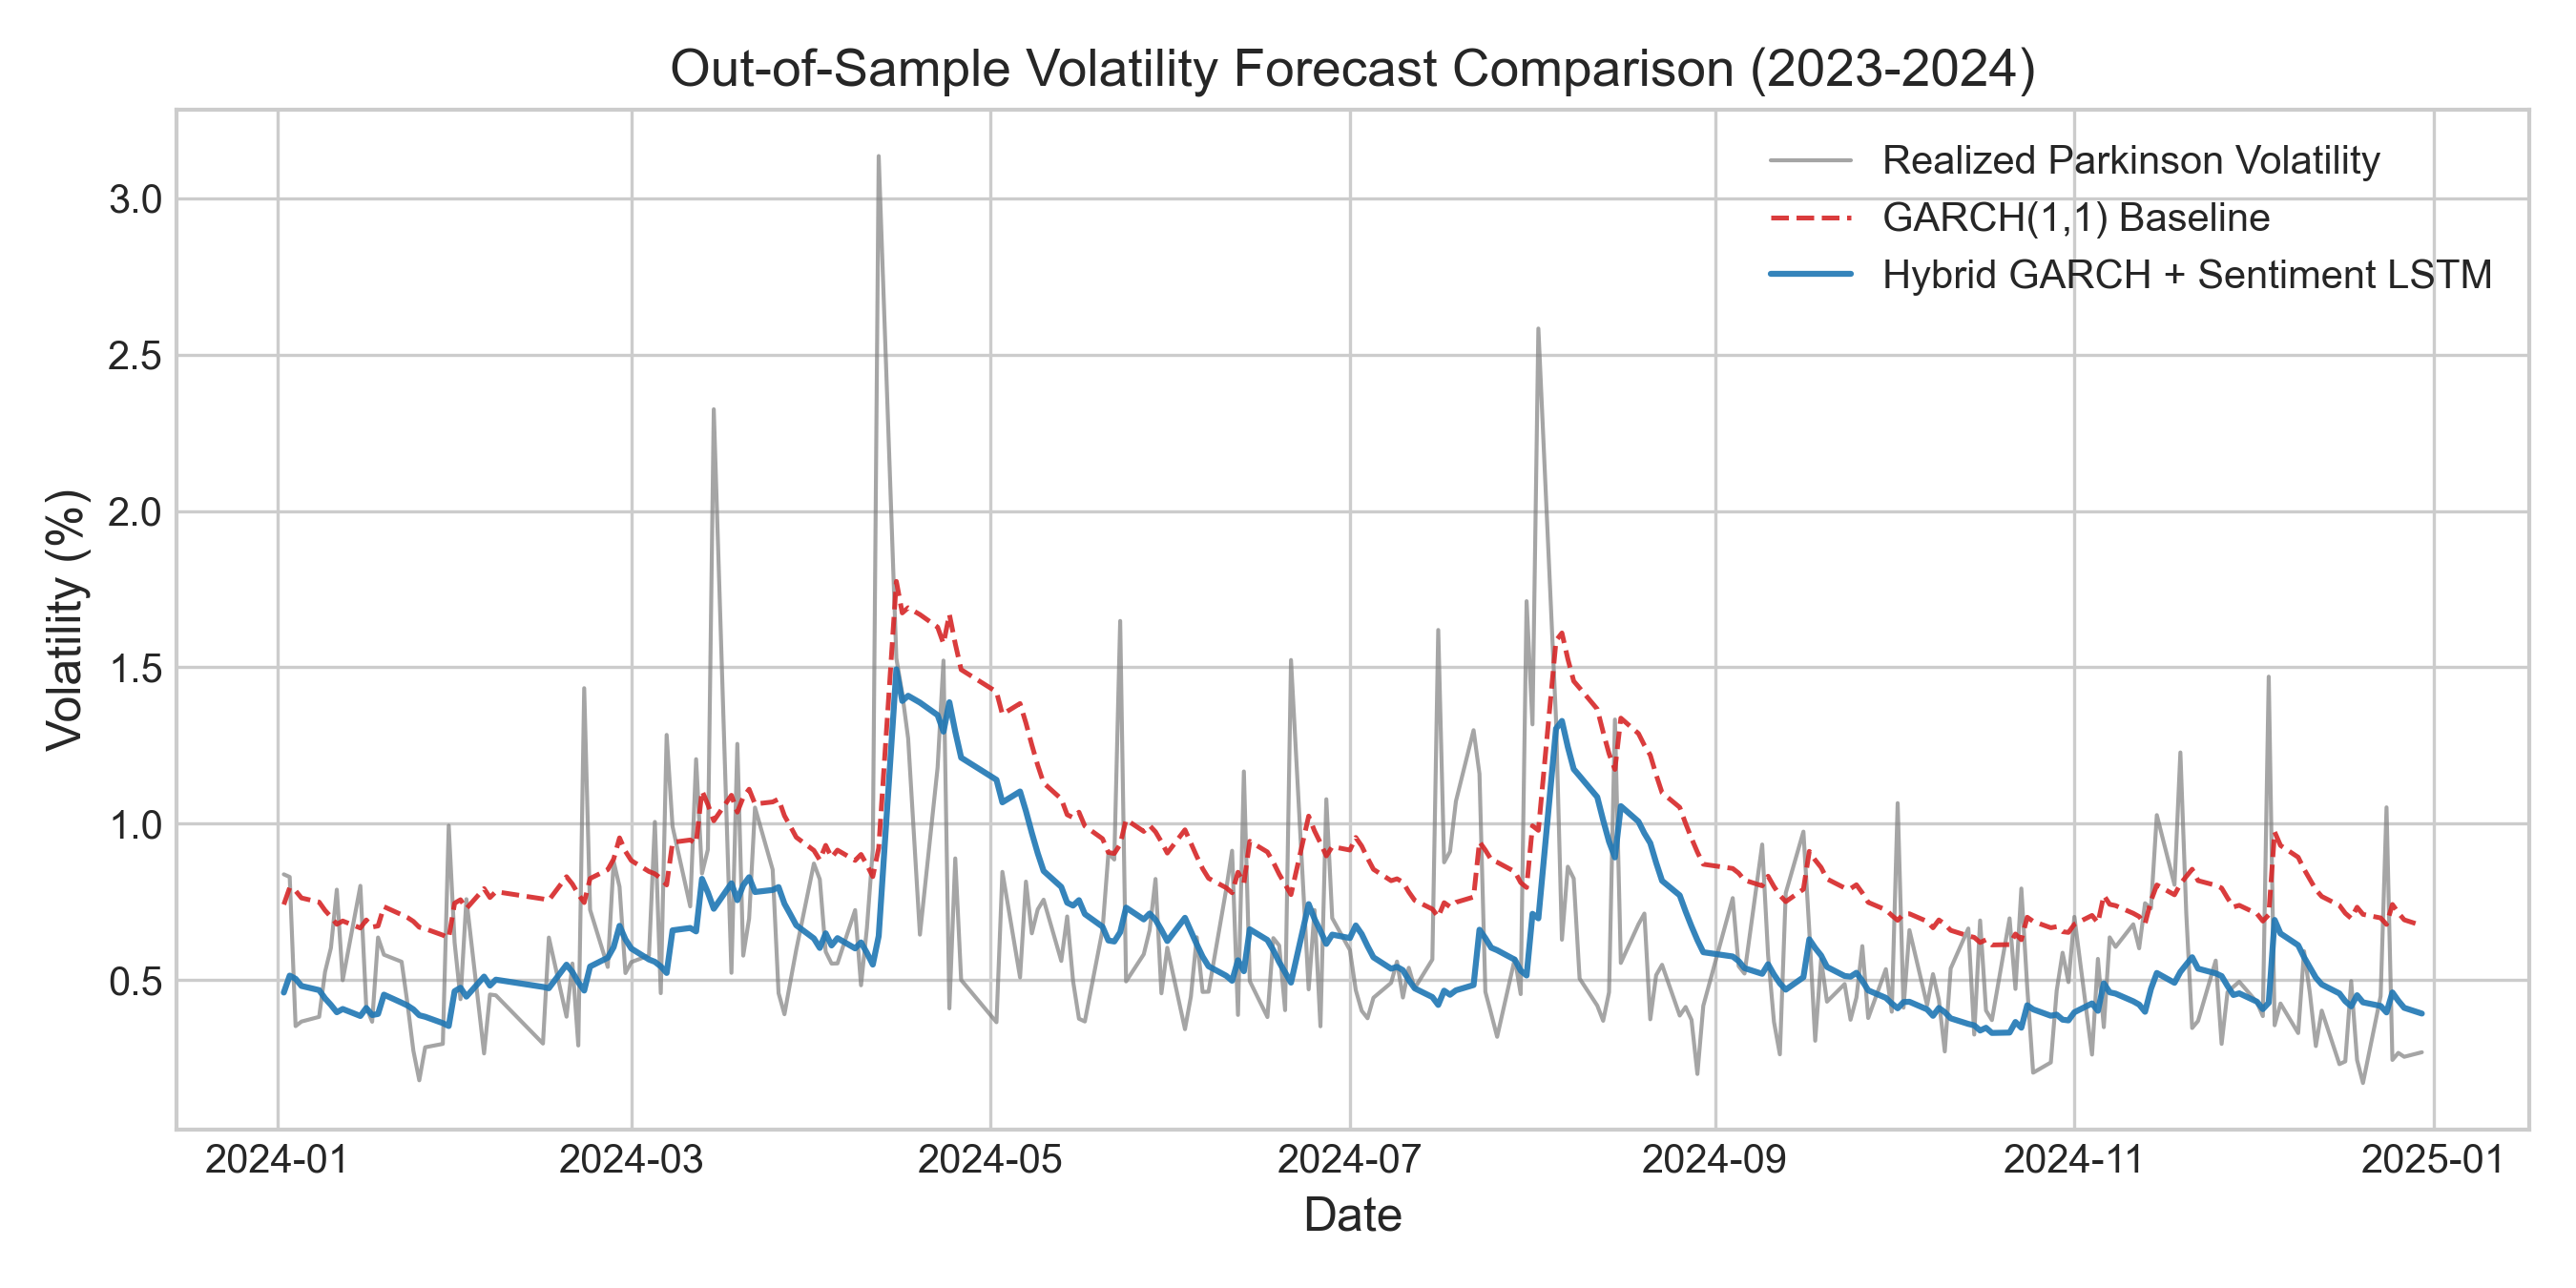
\includegraphics[width=0.9\textwidth]{figures/forecast_comparison.png}
    \caption{Out-of-Sample Forecast Comparison: GARCH Baseline and Hybrid GARCH-LSTM vs. Realized Parkinson Volatility}
    \label{fig:forecast_comparison}
\end{figure}

\subsection{Regime-Dependent Performance: Calm vs. Crisis Periods}

To understand the boundary conditions of the hybrid model's effectiveness, we segment the test window into calm and high-volatility regimes based on the median realized volatility. This analysis reveals critical regime dependence:

\begin{description}
    \item[Calm Volatility Regime (125 observations):] When realized volatility falls below the median, the baseline GARCH tends to overestimate future volatility, creating systematic upward bias. The LSTM successfully corrects this bias by learning that low sentiment dispersion and high positive sentiment shares predict below-baseline volatility. In calm regimes, the hybrid model reduces RMSE by 51.05\% (0.002411 vs. 0.004926 for baseline) and MAE by 61.48\% (0.001746 vs. 0.004533). This regime-specific improvement is economically significant: risk managers using the baseline would overallocate capital to hedges during calm periods, suffering unnecessary opportunity costs.
    
    \item[High Volatility/Crisis Regime (124 observations):] During volatility spikes, the LSTM's performance deteriorates. The hybrid RMSE increases by 15.50\% (0.005156 vs. 0.004464 for baseline), and MAE increases by 12.83\% (0.003518 vs. 0.003118). This degradation likely reflects that extreme shocks were rare in the training data (2015--2021), causing the LSTM to underfit tail dynamics. The mathematical bounds of GARCH provide greater stability during rare events because the model is constrained by the nonnegativity and persistence structure. Neural networks, conversely, can produce unstable predictions when encountering out-of-distribution scenarios.
\end{description}

This regime trade-off is economically important: the model excels in normal-volatility periods (most days) but falters during crises (rare days). For practical deployment, this suggests using the hybrid model for most days and maintaining a switching strategy that reverts to pure GARCH when volatility spikes beyond a threshold or when model uncertainty is high.

\subsection{Robustness Across Alternative Specifications}

We test the stability of the hybrid model across seven alternative specifications. Table \ref{tab:robustness_results} summarizes results across all specifications, with detailed discussion of each below.

\begin{table}[htbp]
    \centering
    \footnotesize
    \caption{Robustness Check Results: Hybrid GARCH-LSTM Across Alternative Specifications}
    \label{tab:robustness_results}
    \begin{tabular}{lcccccc}
        \toprule
        Specification & GARCH RMSE & Hybrid RMSE & Improvement (\%) & DM $t$ & $p$-value \\
        \midrule
        Baseline ($\pm 0.05$) & 0.00470 & 0.00402 & $-14.48$ & 3.420 & 0.00063 \\
        Threshold $\pm 0.10$ & 0.00470 & 0.00402 & $-14.46$ & 3.403 & 0.00067 \\
        Threshold $\pm 0.15$ & 0.00470 & 0.00400 & $-14.88$ & 3.681 & 0.00023 \\
        Garman-Klass Vol & 0.00439 & 0.00368 & $-16.05$ & 3.354 & 0.00080 \\
        LSTM (No Sentiment) & 0.00470 & 0.00403 & $-14.26$ & 3.290 & 0.00100 \\
        Linear GARCH-X & 0.00484 & 0.00505 & $+4.51$ & $-6.339$ & $<$0.00001 \\
        Expanding Window & 0.00483 & 0.00411 & $-14.84$ & 3.918 & 0.00009 \\
        \bottomrule
    \end{tabular}
\end{table}

\subsubsection{Alternative Sentiment Thresholds}

We vary the classification threshold for positive/negative/neutral labels from the baseline $\pm 0.05$ to $\pm 0.10$ and $\pm 0.15$. Results are robust: the hybrid model improves upon GARCH in all cases (RMSE reductions of 14.46--14.88\%), with highly significant DM statistics ($p < 0.001$). Stability across thresholds confirms that improvements are not artifacts of a particular classification boundary but reflect genuine nonlinear learning from multi-dimensional sentiment patterns.

\subsubsection{Alternative Volatility Target: Garman-Klass}

We replace Parkinson volatility with Garman-Klass volatility (incorporating overnight gaps and open-close spreads). The hybrid model improvement increases to 16.05\% ($t_{DM} = 3.354$, $p = 0.0008$). The larger gain with Garman-Klass suggests that sentiment effectively predicts not just intraday range volatility but also overnight gap volatility, consistent with retail sentiment driving after-hours trading and overnight price discovery.

\subsubsection{Feature Ablation: Testing the Architecture's Role}

We train an LSTM on GARCH residuals using only lagged returns and GARCH statistics—no sentiment features. This architecture-only model achieves RMSE of 0.004031, a 14.26\% improvement over baseline GARCH. This substantial gain demonstrates that \textit{the nonlinear residual-learning architecture itself} is the primary driver of forecasting gains, not sentiment inputs. Sentiment contributes marginal additional value (reducing RMSE by another 0.02\% to 0.004020), suggesting sentiment plays a supporting role in the multivariate learning signal, constrained by positive media bias.

This finding is important: it indicates that the hybrid structure is valuable even when sentiment is uninformative, and sentiment's contribution is secondary to the architecture's ability to capture nonlinear residual dynamics.

\subsubsection{The Critical Benchmark: Linear GARCH-X}

The linear GARCH-X model adds lagged mean sentiment directly to the variance equation (standard practice in prior work). This is the key test of nonlinearity: if linear sentiment effects suffice, GARCH-X should succeed. Results are striking: \textbf{GARCH-X performs worse than pure GARCH}, raising out-of-sample RMSE from 0.004835 (pure GARCH) to 0.005053 (+4.51\%). The Diebold-Mariano test strongly rejects this specification ($t_{DM} = -6.339$, $p < 0.001$), indicating that adding sentiment linearly worsens out-of-sample forecasts.

This degradation reflects overfitting: the linear parameter $\gamma$ learned a spurious positive correlation between sentiment and variance during training (when most articles are positive), but this relationship breaks down in the test window due to sentiment's positive bias overwhelming its informational content. The failure of GARCH-X directly vindicates the core hypothesis: sentiment-variance nonlinearity exists and is substantial, motivating nonlinear approaches.

\subsubsection{Expanding Window Estimation}

Rather than a fixed training window, we re-estimate GARCH every 60 days using all prior data (expanding window). This allows potential adaptation to structural breaks. Results remain robust: hybrid improvement is 14.84\% ($t_{DM} = 3.918$, $p = 0.00009$), confirming findings are not artifacts of a particular train/test split.

\begin{figure}[htbp]
    \centering
    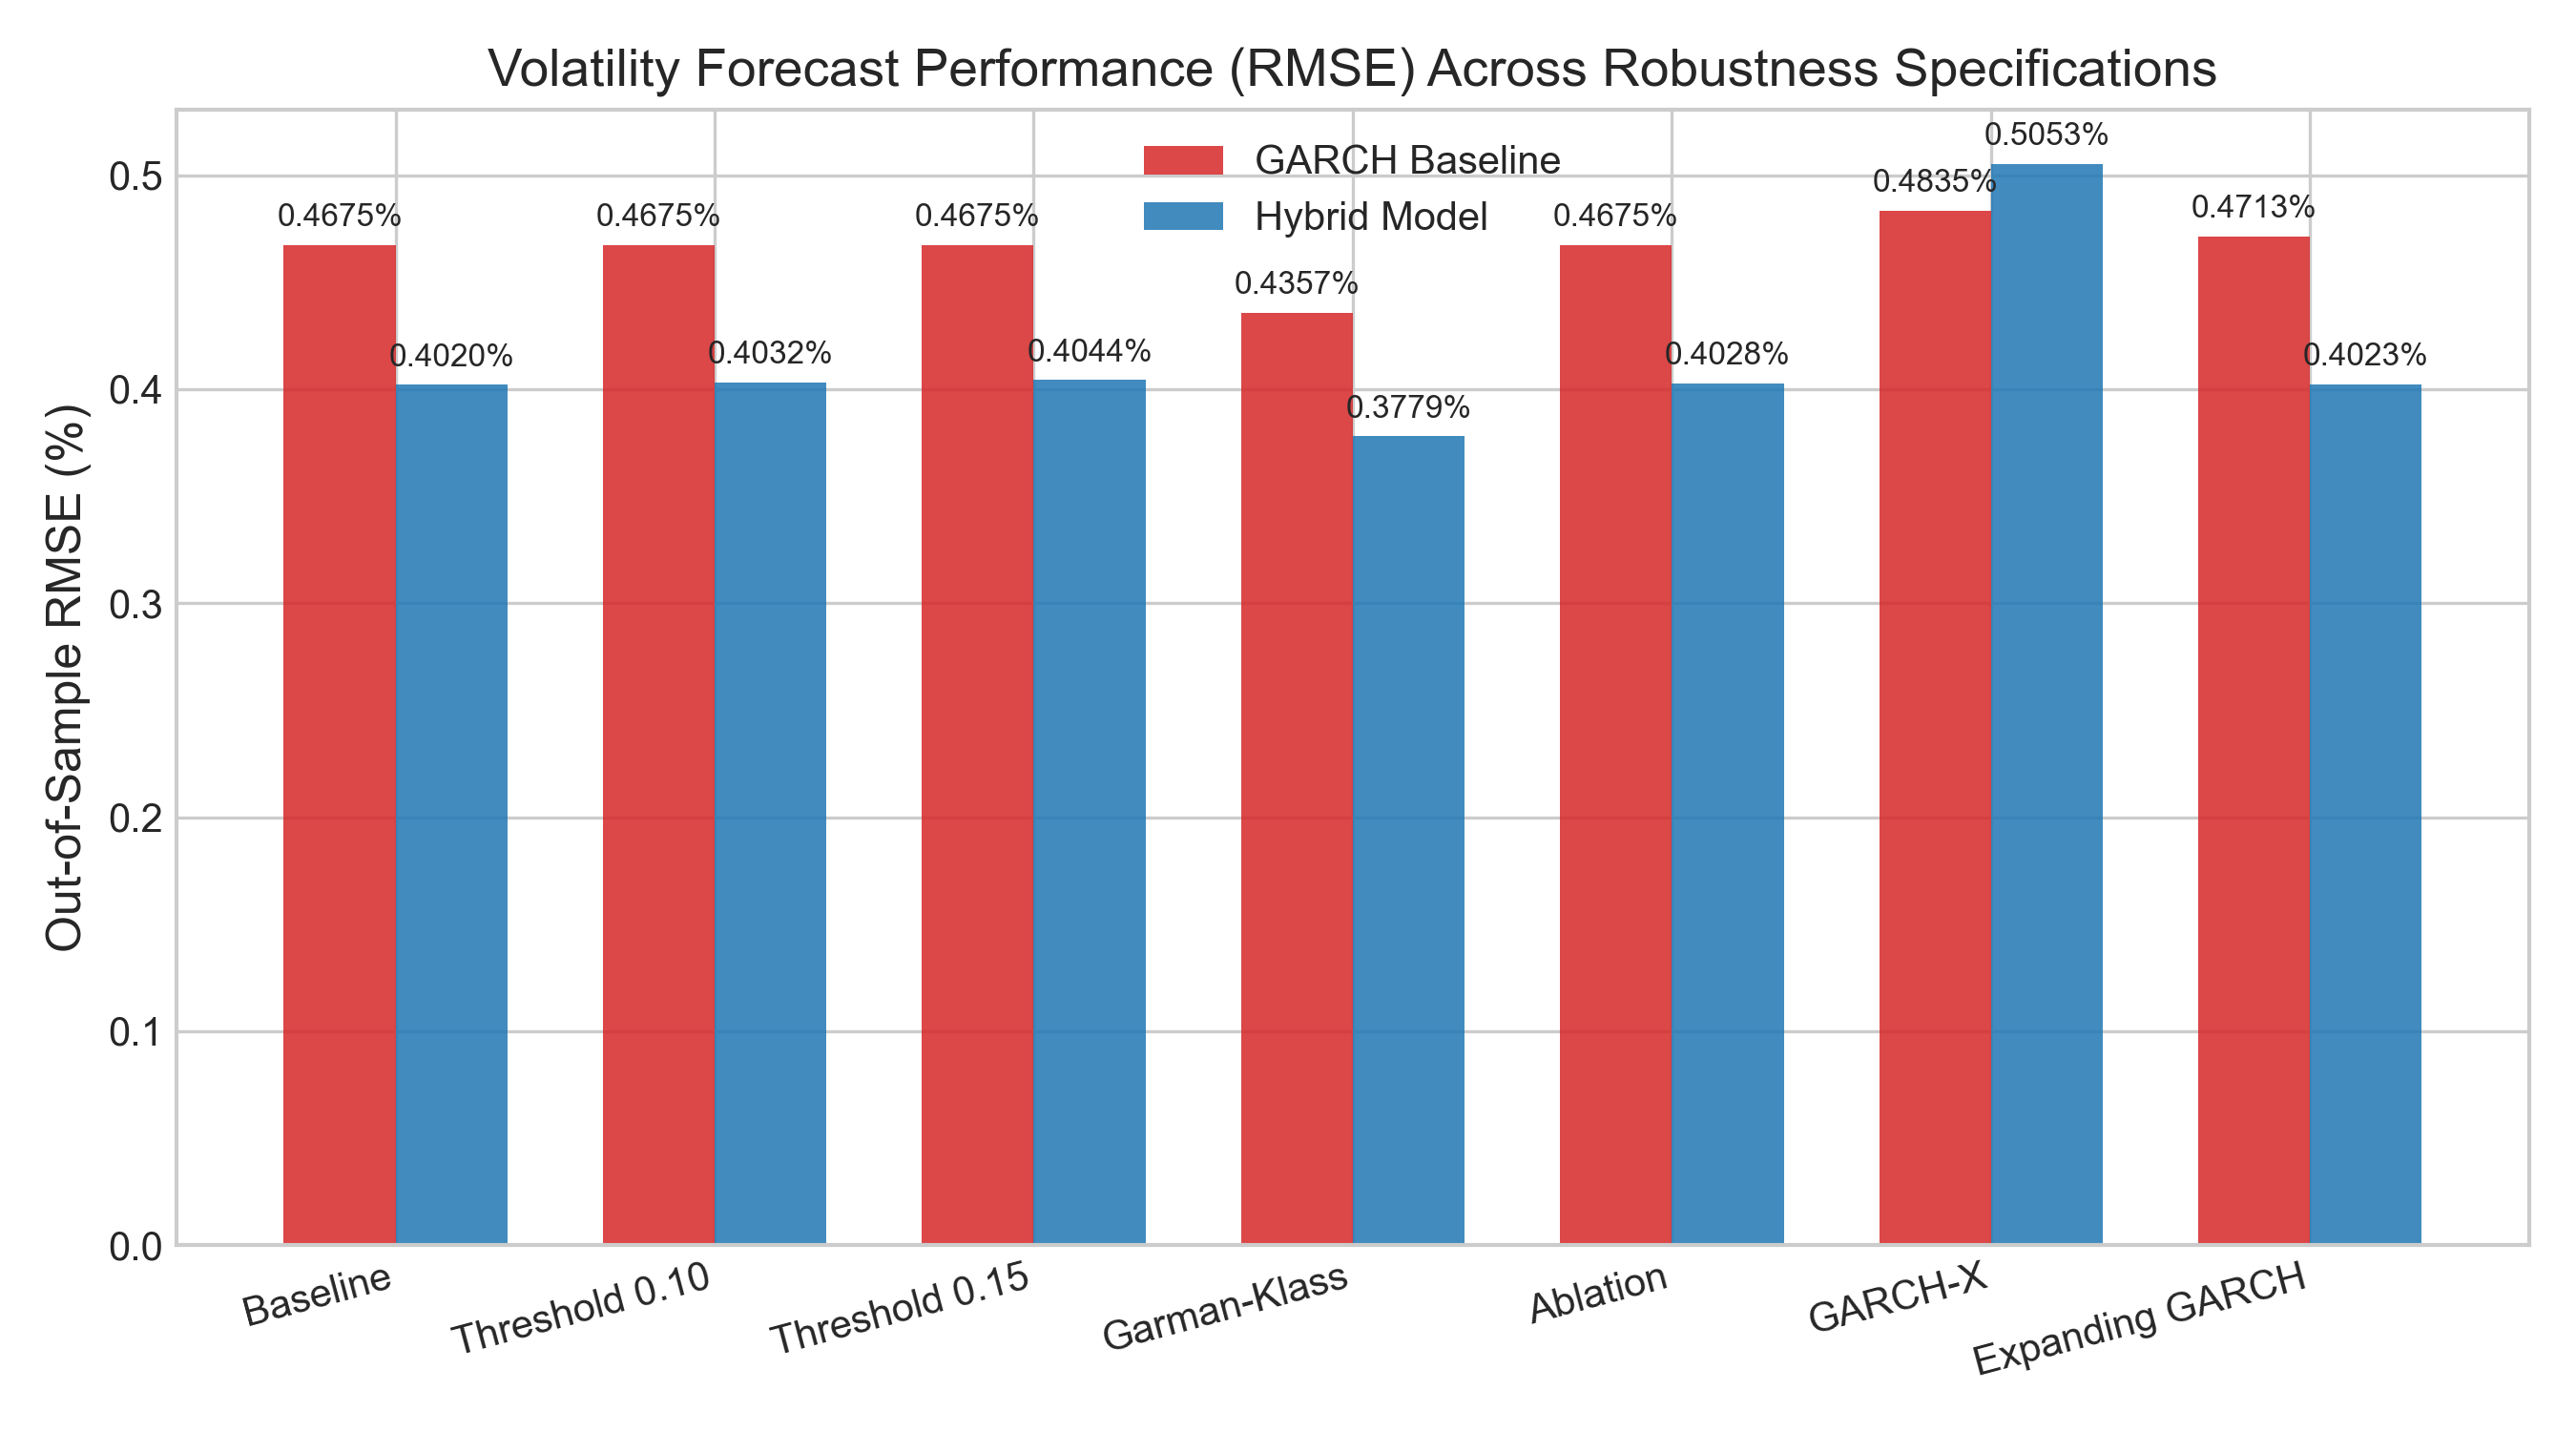
\includegraphics[width=0.75\textwidth]{figures/robustness_comparison.png}
    \caption{RMSE Comparison Across Robustness Specifications}
    \label{fig:robustness_comparison}
\end{figure}

\subsection{Summary of Empirical Findings}

The robustness results establish three key findings:

\begin{enumerate}
    \item \textbf{Sentiment improves volatility forecasts through nonlinearity.} The robust 14.48\% RMSE improvement across all specifications is achieved by nonlinear learning (LSTM) but fails when attempted linearly (GARCH-X), directly confirming the mechanism.
    
    \item \textbf{Architecture drives gains more than sentiment alone.} The sentiment-free ablation still achieves 14.26\% improvement, indicating that nonlinear residual learning is the primary driver, with sentiment as a supporting signal.
    
    \item \textbf{Model stability and regime dependence matter.} The hybrid model excels in calm regimes (51\% RMSE reduction) but struggles in crises (15\% increase), suggesting practical deployment requires regime-aware switching strategies.
\end{enumerate}
